\section{ANDi Tool and Automotive Ethernet in the lab }
\label{sec:network-integration}

This chapter covers the integration of the setup into a larger network.

\subsection{Network Architecture Overview}
% Describe the target network architecture.
In Part 3 of the workshop, the target network architecture for integrating the setup consists of multiple workstations connected via individual MediaGateways to a central MediaGateway. Additionally, a webcam is connected to the central Gateway. Each workstation’s Gateway links through specific ports to the central gateway, creating a star-like topology. This central Gateway manages traffic between the different workstations and shared devices such as the central webcam, enabling communication beyond simple point-to-point connections. This architecture builds on the baseline established in earlier parts, where basic communication paths and VLAN configurations were performed between two devices over a single MediaGateway.

\subsection{Task Report}
The assigned tasks consisted of establishing a functional communication path between the workstation’s MediaGateway and the central MediaGateway, with the objective of accessing the central webcam. The process involved configuring each MediaGateway’s ports with the correct VLAN IDs and ensuring the physical connections to the central MediaGateway are correctly set up. \\\\
\begin{figure}[h]
    \centering
     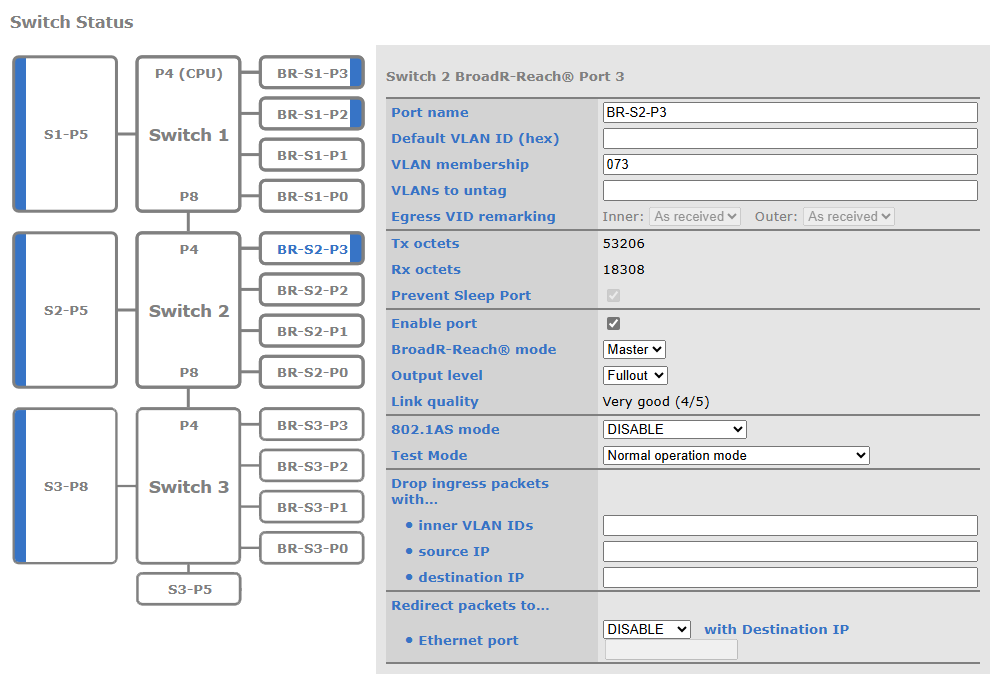
\includegraphics[width=0.8\textwidth]{figures/pictures/vlanconfig2.png}
    \caption{VLAN Configuration.}
    \label{fig:mediagateway_setup4}
\end{figure}\\ After setting up the configuration (Figure 4) a connection to the webcam could not be established, despite everything seemingly being correctly set up. The webcam stayed unresponsive to pings and even the instructor was unsure what was wrong. A restart of the central gateway and the central webcam was issued to troubleshoot, which solved the problem, despite the reason for the error staying unidentified. Post-reboot, connectivity was confirmed via successful ping responses. Remote access to the central webcam could be successfully established through a web browser . Concurrently, network traffic was captured using Wireshark, which verified the presence of correctly tagged Ethernet frames and validated the proper routing of data through the VLANs. 

\subsection{Conclusion}
In this package of Tasks the understanding of working with VLAN was deepened. The proficiency to solving the tasks profited from the gained understanding from prior parts. The unidentified error, that hindered progression of the task, was an obstacle that could be solved through the restart after a long period of tries to work around it.

%To Do: Screenshots einfügen; Netzwerkstruktur einfügen